\documentclass[tikz,border=12pt]{standalone}
\usepackage[T1]{fontenc}
\usepackage{lmodern}
\usepackage{amsmath}
\usetikzlibrary{arrows.meta}
\definecolor{ink}{HTML}{183444}
\definecolor{blue}{HTML}{1B6780}
\definecolor{amber}{HTML}{AD601A}
\begin{document}
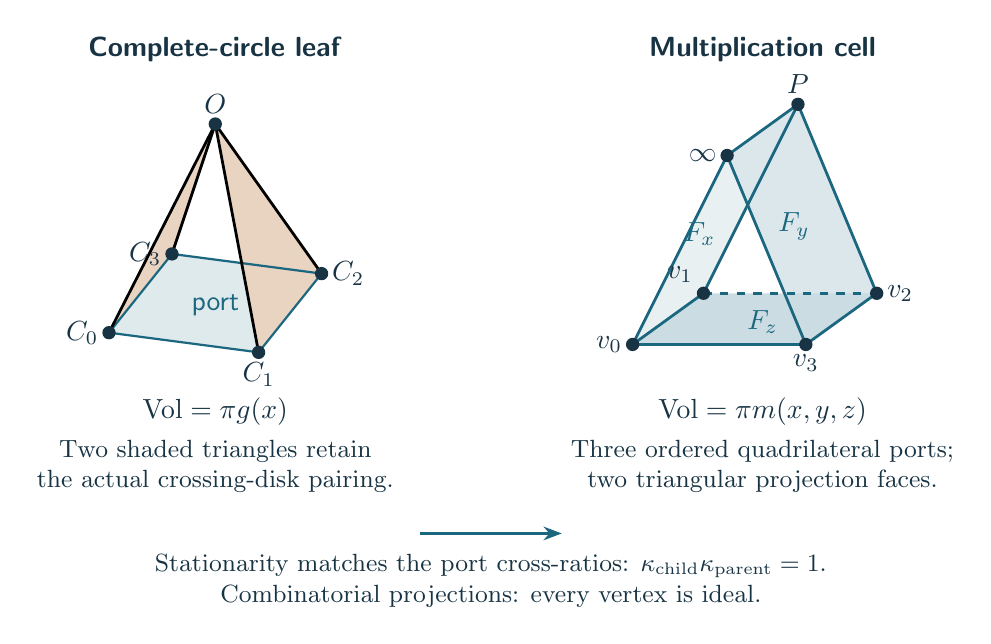
\begin{tikzpicture}[font=\sffamily,text=ink,line width=1pt,
 vertex/.style={circle,fill=ink,inner sep=1.7pt}]
 \begin{scope}[xshift=-3.5cm]
  \node at(0,2.6){\textbf{Complete-circle leaf}};
  \coordinate(O)at(0,1.65);
  \coordinate(C0)at(-1.35,-1.0);\coordinate(C1)at(.55,-1.25);
  \coordinate(C2)at(1.35,-.25);\coordinate(C3)at(-.55,0);
  \fill[blue!14](C0)--(C1)--(C2)--(C3)--cycle;
  \fill[amber!27](O)--(C1)--(C2)--cycle;
  \fill[amber!27](O)--(C3)--(C0)--cycle;
  \draw[blue,thick](C0)--(C1)--(C2)--(C3)--cycle;
  \foreach \p in {C0,C1,C2,C3}{\draw(O)--(\p);\node[vertex]at(\p){};}
  \node[vertex]at(O){};
  \node[above]at(O){$O$};
  \node[left]at(C0){$C_0$};\node[below]at(C1){$C_1$};
  \node[right]at(C2){$C_2$};\node[left]at(C3){$C_3$};
  \node[blue]at(0,-.65){port};
  \node at(0,-2.0){$\operatorname{Vol}=\pi g(x)$};
  \node[font=\small,align=center]at(0,-2.7){Two shaded triangles retain\\the actual crossing-disk pairing.};
 \end{scope}
 \begin{scope}[xshift=3.2cm]
  \node at(.25,2.6){\textbf{Multiplication cell}};
  \coordinate(I)at(-.2,1.25);\coordinate(V0)at(-1.4,-1.15);
  \coordinate(V3)at(.8,-1.15);\coordinate(P)at(.7,1.9);
  \coordinate(V1)at(-.5,-.5);\coordinate(V2)at(1.7,-.5);
  \fill[blue!10](I)--(V0)--(V1)--(P)--cycle;
  \fill[blue!16](I)--(V3)--(V2)--(P)--cycle;
  \fill[blue!23](V0)--(V1)--(V2)--(V3)--cycle;
  \draw[blue](I)--(P)--(V1)--(V0)--(I);
  \draw[blue](P)--(V2)--(V3)--(I);
  \draw[blue](V0)--(V3);\draw[dashed,blue](V1)--(V2);
  \foreach \p in {I,V0,V3,P,V1,V2}{\node[vertex]at(\p){};}
  \node[left]at(I){$\infty$};\node[above]at(P){$P$};
  \node[left]at(V0){$v_0$};\node[above left]at(V1){$v_1$};
  \node[right]at(V2){$v_2$};\node[below]at(V3){$v_3$};
  \node[blue]at(-.55,.25){$F_x$};\node[blue]at(.65,.35){$F_y$};
  \node[blue]at(.25,-.87){$F_z$};
  \node at(.25,-2.0){$\operatorname{Vol}=\pi m(x,y,z)$};
  \node[font=\small,align=center]at(.25,-2.7){Three ordered quadrilateral ports;\\two triangular projection faces.};
 \end{scope}
 \draw[blue,thick,->,>=Stealth](-.9,-3.55)--(.9,-3.55);
 \node[font=\small,align=center]at(0,-4.15)
 {Stationarity matches the port cross-ratios: $\kappa_{\rm child}\kappa_{\rm parent}=1$.\\
  Combinatorial projections: every vertex is ideal.};
\end{tikzpicture}
\end{document}
